\subsection{Motivation}
\noindent According to the latest report from Home Security Heroes, the number of deepfake contents in the year 2023 has risen to 96,000, representing a growth of approximately 550\% compared to 2019. Even in technologically advanced regions such as the United Kingdom, only 32.9\% of the population expresses confidence in their ability to discern deepfake content. Notably, the corresponding figure for Nepal is considerably lower. Given this circumstance, the necessity to deploy an deepfake detection tool becomes apparent, functioning as a pivotal tool to address crimes and theft associated with deepfakes and  restrict the propagation of misinformation.
\begin{figure}[h]
    \centering
    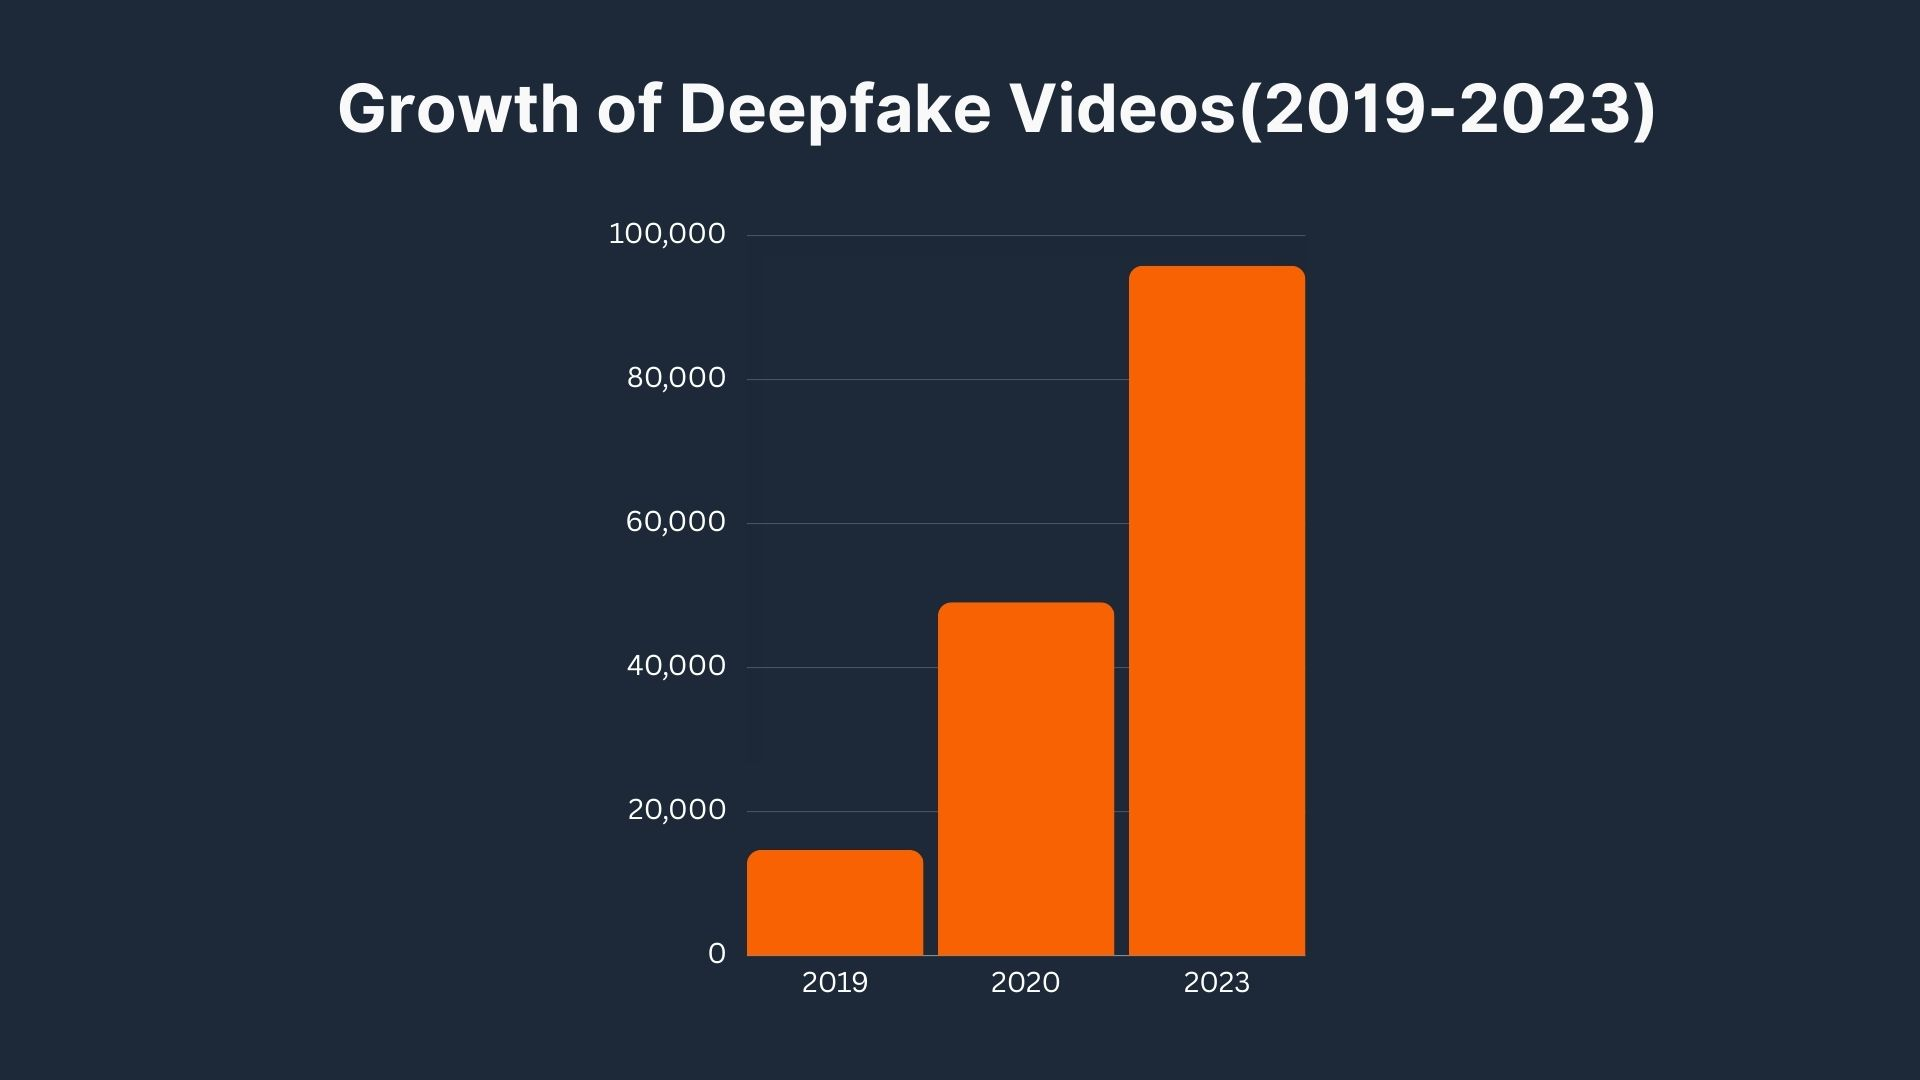
\includegraphics[width= 5.5in ]{img/chart.jpg}
    \caption{Deepfake videos growth over time}
\end{figure}
